\section{Numerical verification}\label{sec:exp}

In this section, we conduct experiments to verify our theoretical results, i.e., Theorem~\ref{theo:ntk0}. Specifically,  we aim to verify that if the network width grows linearly with the number of training samples, the minimum eigenvalue of the NTK is bounded from a positive constant. 

Our experimental setup is as follows: we consider a 3-layer (2-hidden layer) fully-connected neural network with Sigmoid/Tanh activation function, and whose hidden layers have the same width $m$. We consider $m \in \{200, 300,..., 4000\}$. We train the network over $n$ data points, with each data point being drawn i.i.d. from $\mathcal{N}(0,\I_{100})$. We let the number of data points be the same as the width, i.e., $n=m$. We report the average of the minimum eigenvalue of the NTK out of 3 independent runs (i.e., each run uses the same training data but has different random initialization of the weights).

From Figure~\ref{fig:min_ntk} we can see that across all experiments, the minimum eigenvalue of NTK stays persistently positive. Furthermore, as $m$ (as well as $n$) is made sufficiently large, the minimum eigenvalue of NTK shows only a mild decrease in the average value which mostly flattens out as $m$ (and $n$) increases. In summary, the minimum eigenvalue of the NTK can be lower bounded by some constant. 


\begin{figure}[h!] 
\centering
% \subfigure[CIFAR-10: $\|\bar{\g}_t\|_2$ over iterations.]{
%  \includegraphics[width =  0.45\textwidth]{Updated_NeurIPS22/figs/cifar-training_curve.png}
%  }
% \subfigure[CIFAR-10: Minimum $\|\bar{\g}_t\|_2$ vs.~width.]{
%  \includegraphics[width =  0.45\textwidth]{Updated_NeurIPS22/figs/cifar-min-norm.png}
%  }   \\
%  \subfigure[MNIST: Minimum $\|\bar{\g}_t\|_2$ vs.~width.]{
%  \includegraphics[width =  0.45\textwidth]{Updated_NeurIPS22/figs/mnist-min-norm.png}
%  }  
\subfigure[$\lambda_{\min}(K)$ vs.~width.]{
 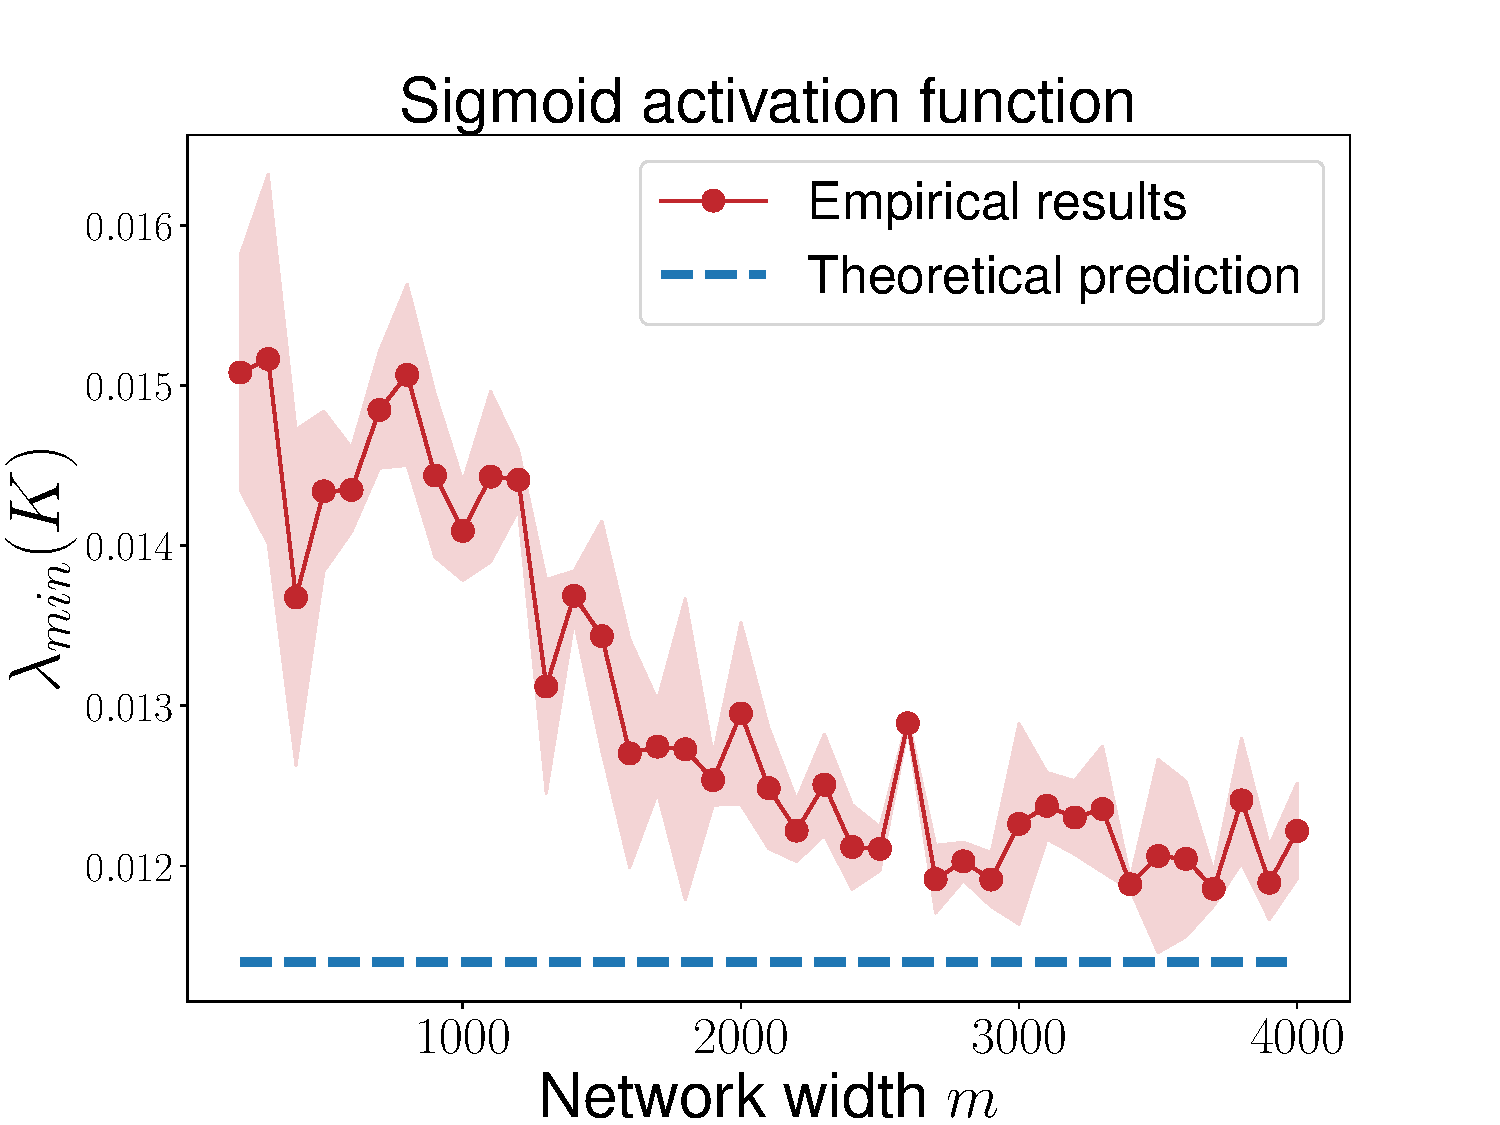
\includegraphics[width =  0.42\textwidth]{fig/min_eig_sigmoid.pdf}
 } \\
\subfigure[$\lambda_{\min}(K)$ vs.~width.]{
 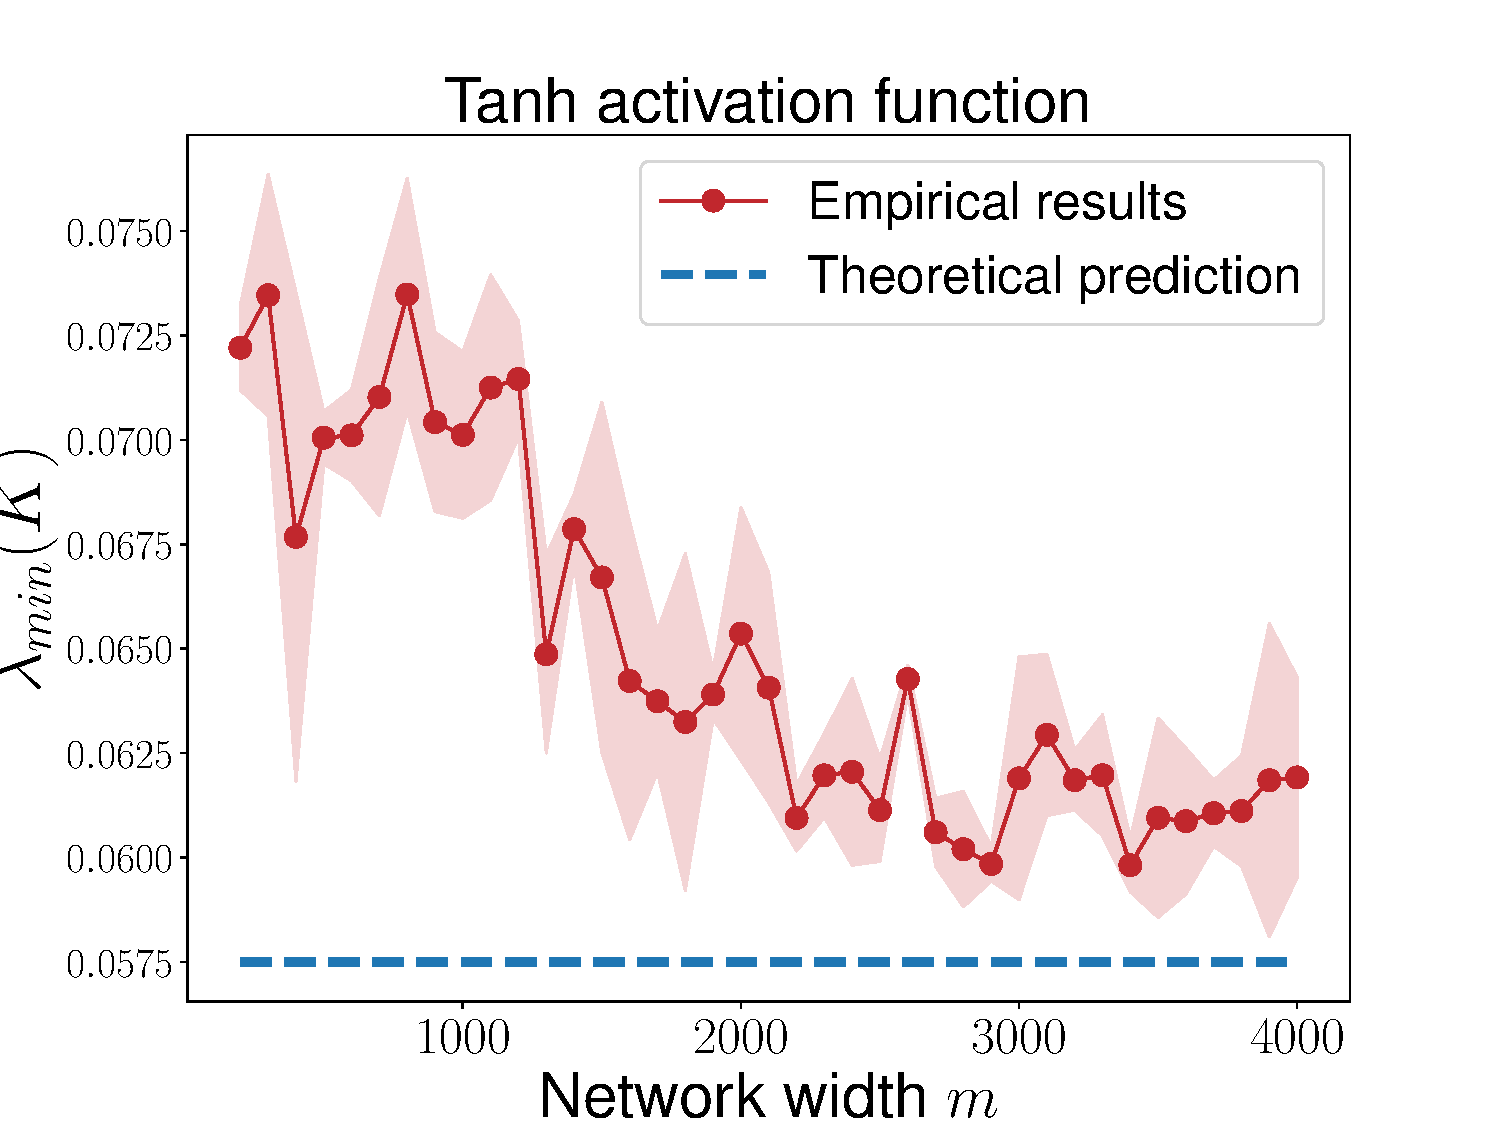
\includegraphics[width =  0.42\textwidth]{fig/min_eig_tanh.pdf}
 } 
\caption[]{Positive $\lambda_{\min}(K)$ with linear width. In the experiments, we train a 3-layer fully-connected neural network with Sigmoid/Tanh activation functions whose width has the same numerical value as the number of data points. Each curve is the average of 3 independent runs.\label{fig:min_ntk}}
\end{figure}